%Version up to 8 feb. In the following I will imeplemtn ulrikes suggestions, including re-structuring the paper to follow the framework flow better. I will also implement Lyles suggestions and he might also edit the intro.

%  \documentclass[12pt, onecolumn, a4paper]{article}
% \documentclass[reprint,showpacs,amsmath,superscriptaddress,amssymb,aps,floatfix,nolongbibliography]{revtex4-2}
\documentclass[reprint,onecolumn,superscriptaddress,showpacs,amsmath,amssymb,aps,floatfix]{revtex4-2}
\usepackage[utf8]{inputenc}
\usepackage[T1]{fontenc}
\usepackage[english]{babel}
\usepackage{amsmath}
\usepackage{graphicx}		
\usepackage{natbib}
\usepackage{textcomp}
\usepackage{gensymb}
\usepackage[hidelinks]{hyperref}
\usepackage{xcolor}
\usepackage{siunitx}
\usepackage{mathrsfs}
\usepackage{multirow}
\usepackage{amsthm}
\usepackage{float}
\theoremstyle{definition}
\newtheorem{definition}{Definition}[section]
\newcommand{\kl}[1]{\textcolor{red}{#1}}
% \newcommand{\figref}[2]{Fig. #1}{#2}
\newcommand{\Emph}[1]{\textbf{#1}}
\graphicspath{{figs-perspective/}}
\newcommand*{\everymodeprime}{\ensuremath{\prime}} 
% \usepackage{printlen} %textwidth = 510pt
% \printlength\columnwidth
% \linespread{1.5} %Increase baselineskip (for Ulrike)


% idea: send to https://journals.plos.org/ploscompbiol/s/other-article-types. Mximum length: 2500 words!

\begin{document}
\title{Towards a unified framework for metastability in neuroscience}
\author{K. L. Rossi}
\affiliation{Theoretical Physics/Complex Systems, ICBM, Carl von Ossietzky University Oldenburg, Oldenburg, Lower Saxony, Germany}
\author{R. C. Budzinski}
\affiliation{Department of Mathematics, Western University, London, Ontario, Canada}
\affiliation{Western Institute for Neuroscience, Western University, London, Ontario, Canada}
\affiliation{Western Academy for Advanced Research, Western University, London, Ontario, Canada}
\author{B. R. R. Boaretto}
\affiliation{Institute of Science and Technology, Federal University of São Paulo, São José dos Campos, São Paulo, Brazil}
\author{E. S. Medeiros}
\affiliation{Theoretical Physics/Complex Systems, ICBM, Carl von Ossietzky University Oldenburg, Oldenburg, Lower Saxony, Germany}
\author{L. Muller}
\affiliation{Department of Mathematics, Western University, London, Ontario, Canada}
\affiliation{Western Institute for Neuroscience, Western University, London, Ontario, Canada}
\affiliation{Western Academy for Advanced Research, Western University, London, Ontario, Canada}
\author{U. Feudel}
\affiliation{Theoretical Physics/Complex Systems, ICBM, Carl von Ossietzky University Oldenburg, Oldenburg, Lower Saxony, Germany}


\begin{abstract}
The brain is commonly proposed to have metastable dynamics, typically thought of as a regime with a succession of long-lived states. Evidence from a wide variety of experiments has accumulated to suggest important cognitive and sensory roles for this regime. However, a general, unified framework in neuroscience for studying metastability is still unavailable, as evidenced for instance in the lack of a consistent definition of the term in the literature. In this perspective, we provide a step towards unifying the definitions, observations, and mechanisms for metastability in neuroscience into a single framework. We take insights from dynamical systems theory by examining several universal dynamical mechanisms capable of generating metastable behavior, and propose a simple definition of metastability that encompasses views in neuroscience and dynamical systems theory. This definition works as an umbrella term that encompasses most other definitions in the literature as distinct subtypes, which allows us to clarify their unique properties and functional roles. With this, we expand and deepen the current discussions on the dynamical mechanisms for metastability. We believe that this framework is an important step towards improving our understanding of metastability in the brain, which can lead to the development of better tools to control and predict its behavior. 
\end{abstract}

\maketitle

\section{Metastability is important, but what is it actually?}
The brain typically operates in a regime that switches between states over time, with each state appearing stable for some duration before transitioning to another state \cite{michel2017eeg, vandeville2010eeg, lehmann1987eeg, jones2007natural, lacamera2019cortical, mazzucato2019expectation, recanatesi2021metastable, brinkman2022metastable, abeles1995cortical, seidemann1996simultaneously, jercog2017updown, luczak2007sequential, mazor2005transient, sasaki2007metastability, mashour2020conscious, dehaene2005ongoing, hudson2014recovery, tognoli2014metastable, popa2009constracting, curtis2015initiation, fernandez2020sleep}.  This regime is often called \textit{metastability}, and each state is called a metastable state. It occurs for several species, task paradigms, and experimental apparatus, and has been associated to several functional roles (see Fig. \ref{fig:observationsmetastability} for more details). Examples of this behavior are the sleep stages \cite{yetton2018quantifying, fernandez2020sleep} and EEG microstates \cite{michel2017eeg}.

Despite the ubiquity and importance of metastability, a unified framework to understand and describe its many facets is still unavailable. One instance of this is the current lack of agreement about the exact meaning of metastability: a close look into the literature reveals several disagreements about what metastability is, and under which circumstances it can arise (see Fig. \ref{fig:definitionsmetastability}B). This hampers systematic comparisons between works and also constrains studies on the dynamical mechanisms for this behavior. 

In this perspective, we propose to overcome this issue by providing important steps towards a framework that unifies observations and definitions of metastability. The key to do this is to use knowledge from the theory of dynamical systems, in which dynamical regimes similar to metastability are well-known. With its insights, we first propose a general definition of metastability that acts as an umbrella term encompassing its various observations and definitions in both neuroscience and dynamical systems theory. The current definitions of metastability then fit neatly into a subtype of this general metastability, which allows the framework to deal with the specificities of each subtype while maintaining a broad, high-level, view of the phenomenon. This unified view allows us to deepen and expand the current discussions on mechanisms for metastability in the brain by showing that many more mechanisms are possible and by bringing more insights into previously proposed mechanisms. 

To do this, we first provide examples of observations and definitions of metastability in the literature, then present some universal mechanisms that can account for observations of metastability in neuroscience using as didactic examples low-dimensional, paradigmatic, systems. These give us insights to propose the unifying definition of metastability and discuss its mechanisms. We believe that the unified framework proposed here is a significant step towards developing a better characterization and understanding of metastability in the brain. Further, the better understanding of mechanisms can then aid in developing better tools to control and predict brain behavior.


\section{Observations of metastability in the brain}
To start, we now describe various experiments that have helped to establish metastability as an important dynamical regime for the brain. We focus here on metastability characterized by successions of long-lived states, following a common view in the literature, and which we argue later is more meaningful. With these examples, we would also like to draw attention to what a \textit{state} is. As the examples show, the states observed depend on the measurement techniques used to extract the data and on the analysis techniques used to identify the states from the data, so that the term is very general, and can depend on techniques of each individual work. Despite this, states can be jointly thought of as epochs of distinct dynamics, with some stationarity in their features.
Furthermore, we wish to remark that metastable states can be observed in resting and stimulus-driven paradigms, as Fig. \ref{fig:observationsmetastability} details for each example. Similarly, the figure also mentions whether the states repeat over the time series or not, properties which are used later to define subtypes of metastability.

To start, Fig. \ref{fig:observationsmetastability}A shows time-series of electroencephalography (EEG) measurements performed in resting humans with eyes closed (taken from \cite{michel2017eeg}). Colors indicate \Emph{EEG microstates}, identified from the spatial configuration of the electric potential amplitude of each electrode. These microstates remain almost stationary for roughly $\SI{100}{\milli\second}$ \cite{vandeville2010eeg, lehmann1987eeg}, and then give way to other microstates. Microstates are proposed to play an important role in cognition and perception \cite{vandeville2010eeg, lehmann1987eeg, michel2017eeg}.

Figure \ref{fig:observationsmetastability}B-E show results based on firing rates of neurons.
Figure \ref{fig:observationsmetastability}B shows exemplary sequences of states adapted from \cite{brinkman2022metastable}. The states are characterized by roughly stationary behavior in the firing rates of neurons in the gustatory cortex of rats, and are identified via the technique of \Emph{hidden Markov model} (HMM). Each state lasts for roughly an order of magnitude longer than the transitions between them \cite{jones2007natural, lacamera2019cortical, mazzucato2019expectation, recanatesi2021metastable, brinkman2022metastable}. This is observed during both spontaneous and stimulus-evoked activity, and the sequence of such states is shown to encode the stimuli \cite{lacamera2019cortical, mazzucato2019expectation} presented to the animals. These states are proposed to serve as a ``substrate for internal computations" in the brain \cite{lacamera2019cortical}. Similar results have also been reported in the frontal cortex of monkeys during a delayed localization task \cite{abeles1995cortical, seidemann1996simultaneously}.

Figure \ref{fig:observationsmetastability}C shows sequences of sustained firing (significant activity, \Emph{UP states}) and silence (\Emph{DOWN states}) in the firing rates of the deep layers of the somatosensory cortex of urethane-anesthetized rats (adapted from \cite{jercog2017updown}). Each state lasts for a significant time, with quick transitions between them \cite{jercog2017updown}. These states are ubiquitously observed in spontaneous activity \cite{luczak2007sequential, jercog2017updown}. 

In Fig. \ref{fig:observationsmetastability}D, the firing rate of neurons in slice cultures of the hippocampal CA3 region was found to evolve also as sequences of discrete, long-lasting states, separated by quick transitions \cite{sasaki2007metastability}. The figure was taken from \cite{sasaki2007metastability} (Copyright 2007 Society for Neuroscience). Each state is identified by clustering algorithms applied to the space spanned by the principal components obtained from Principal Component Analysis (\Emph{PCA}) of the firing rates. The figure shows the raster plot of the firing, and the total activity, with colors denoting each state \cite{sasaki2007metastability}.

Interesting work by Mazor and Laurent \cite{mazor2005transient} (not included in the figure) measured the firing rate of neurons in the antennal lobe of locusts as the animals were presented with a variety of pulses of odors. For long pulses (lasting more than $\SI{1}{\second}$), the activity passed through three different phases: an on-transient phase (lasting $1$-$2$ $\SI{}{\second}$) towards a fixed point (with stable activity or silence), stable for at least $\SI{8}{\second}$, then an off-transient lasting a few seconds as activity returned to baseline, which is also stationary and thus also considered a fixed point. The trajectory is considered as a transition from the fixed point baseline towards the odor-specific fixed point. 
% The figure shows the raster plots of firing rates (top) and the total activity (bottom) on the left and an illustration of the trajectory on the right \cite{mazor2005transient}. 
Interestingly, optimal stimulus encoding occurred during the transients, not the fixed point  \cite{mazor2005transient}. For short pulses, the odor-specific fixed point was entirely skipped.


Figure \ref{fig:observationsmetastability}E shows that metastable states also occur in the context of consciousness. The global neuronal workspace theory of consciousness proposes that we become conscious of a certain object (e.g. a stimulus) when the representation of that object is broadcast from local processing regions into a variety of spatially distributed regions, which form the global workspace \cite{mashour2020conscious}. This global broadcast is known as \Emph{ignition}, and is achieved through the sustained firing of the involved areas; this is shown in panel E for the local-field potential (LFP) and spikes in area D2 of the model studied in \cite{dehaene2005ongoing}. The figure is adapted from \cite{dehaene2005ongoing}. The activity of workspace neurons is thus characterized by discrete episodes of spontaneous coherent activation, with sustained firing, and quick transitions between them \cite{michel2017eeg}.

Another work (not included in the figure) has also found that the power spectrum of LFP recordings in rats progresses as a sequence of relatively stationary states lasting for some time before rapidly transitioning to other states \cite{hudson2014recovery} (see e.g. Fig. 2 of \cite{hudson2014recovery}). This was observed as the rats recovered consciousness, when the concentration of an anesthetic was progressively decreased. The authors argue that the existence of well-defined metastable states is crucial for the fast recovery of consciousness \cite{hudson2014recovery}.

Figure \ref{fig:observationsmetastability}F shows the swim motor pattern in intracellular recordings of two neurons that belong to the swim central pattern generator of the mollusk \textit{Tritonia} \cite{sakurai2016recruitment} (adapted from \cite{sakurai2016recruitment}). These neurons respond to stimulation in a nerve called PdN3 by \Emph{bursting}. These bursts are phenomenologically similar to that later shown in Fig. \ref{fig:mechanismsmetastability}E (though their mechanisms might differ), and show the alternation between periods of sustained  firing and periods of silence. Central pattern generators \cite{marder2001central} contain various examples of metastable states. 

Additionally, we remark that several other regimes could be mentioned in this section, such as the case of seizures \cite{curtis2015initiation, babloyantz1986low}, whose initiation and termination occur quite quickly, sleep spindles \cite{fernandez2020sleep}, transient patterns of circular waves that travel across the cortex repeatedly occur over sleep that aid in the consolidation of memories \cite{muller2016rotating}, and the phases of local-field potentials in cats at rest \cite{tognoli2014metastable, popa2009constracting}. Additional references are also discussed in \cite{tsuda2009hypotheses}.

We also note that some works mentioned previously may have not necessarily used the term metastability in their respective manuscripts. Also, we note that some works interpret metastability differently than the idea of long-lasting states, and they were not included here.
%
\begin{figure*}[hbt]
    \centering
    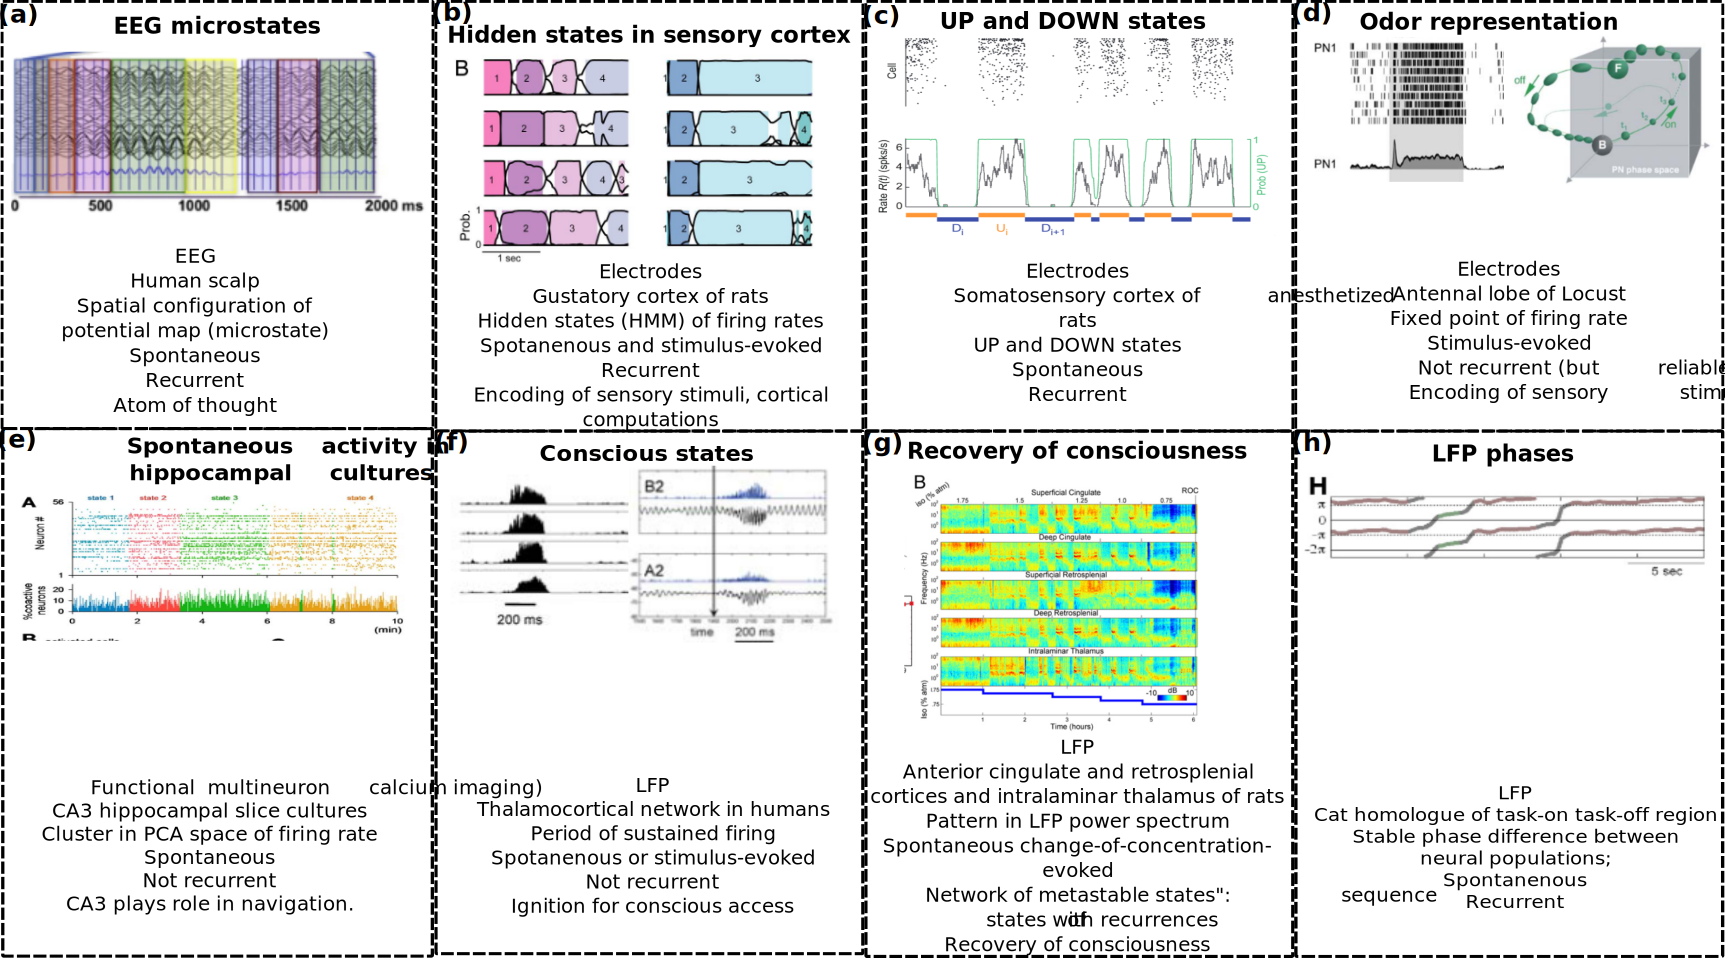
\includegraphics[width=\textwidth]{observationsmetastability.pdf}
    \caption{\textbf{Various observations reveal regimes in which brain activity evolves as a sequence of well-defined states that are transient but long lived.} Each panel corresponds to one observation, taken from references cited and better explained in the main text, and has a classification of the behavior into the subtypes of metastability we define in the text.
    }
    \label{fig:observationsmetastability}
\end{figure*}

\section{Current definitions of metastability}
As previously mentioned, despite the importance and widespread interest in metastability, its definition is not clear in the literature: several studies work on distinct definitions, with their own specificities. This is illustrated in Fig. \ref{fig:definitionsmetastability}.

For reference, we start with a typical definition of metastability in physics, especially statistical and quantum physics. There, a metastable state is an equilibrium, in which the system can stay for an indefinitely long time until sufficiently strong perturbations, or quantum fluctuations, take it into another state \cite{olivieri2005large, bovier2009metastability, makela1997metastable}. In terms of an energy landscape, a system tends to minimize its energy, such that the stable equilibrium correspond to the global minimum in this landscape. There, metastable states correspond to local minima of energy, and a succession of metastable states would appear as shown in section "Variability in energy landscape" of Fig. \ref{fig:definitionsmetastability}. In dynamical systems theory, metastability generally refers to long-lived states \cite{yorke1979metastable, bittracher2018transition}.

% Metastability was already in the 1970s also mentioned in the dynamical systems literature as states that last for a long time, appearing stable, but are ultimately unstable \cite{yorke1979metastable}.

These ideas were adapted into neuroscience by Kelso and colleagues \cite{kelso1991an} and subsequently branched into several definitions. Some of these are presented in Fig. \ref{fig:definitionsmetastability}: variability in activity patterns \cite{friston1997transients, friston2000transients, varela2001brainweb, roberts2019metastable} (panel A); variability of states \cite{mazzucato2015dynamics, lacamera2019cortical, afraimovich2010longrange, alderson2020metastable, lee2017linking, vasa2015effects, hellyer2014control, naik2017metastability, rabinovich2008transientcognitive, cavanna2018dynamic, werner2007metastability, bhowmik2013metastability} (panel B); variability in regions of state space \cite{hudson2017metastability, graben2019metastable} (panel C); variability of synchronization \cite{cabral2011role, deco2017dynamics, deco2016metastability, poncealvarez2015restingstate, aguilera2016extended} (panel D); variability in an energy landscape \cite{gili2018metastable, cavanna2018dynamic, aguilera2016extended} (panel E); integration and segregation of neural assemblies \cite{deco2015rethinking, fingelkurts2001operational, tognoli2014metastable, tognoli2014enlarging, bressler2016coordination, kelso2012multistability, hellyer2015cognitive} (panel F). Most of these therefore think of metastability as a succession of some feature of the dynamics (which might be called activity pattern, states, etc.) The main difference in this case comes from what is considered to be a state, and whether they are long-lived or not. 


There are also several distinct views in neuroscience about the mechanism for the transitions between the states (Fig. \ref{fig:definitionsmetastability}C). Some works argue that the transitions need to be spontaneous, occurring in autonomous systems \cite{sasaki2007metastability, kelso2012multistability, roberts2019metastable, fingelkurts2008brainmind, cavanna2018dynamic}, while others argue that the transitions need to be externally induced (non-autonomous systems) \cite{jercog2017updown, hudson2017metastability}. Further, others argue that both are possible \cite{brinkman2022metastable, friston2000transients, lacamera2019cortical}. Each mechanism has distinct but important functional roles: spontaneous metastability enables transitions between states without expenditure of energy, and guarantees a system does not get stuck in the same state \cite{ito2008dynamics} for inducing the transitions; forced metastability is important for direct control of the transitions, and in stimulus-evoked cases. 
%
\begin{figure*}[htb]
    \centering
    \includegraphics[width=\textwidth]{definitionsmetastability.pdf}
    \caption{\textbf{Definitions of metastability common in the neuroscience literature.} A common theme among these is the presence of transitions between certain aspects of the system's dynamics (e.g. between activity patterns). The upper part of the figure illustrates what these aspects are in each definition, and the bottom part shows characteristics of the transitions. Further details are available in the main text.}
    \label{fig:definitionsmetastability}
\end{figure*}

\section{A unifying definition of metastability}
In this perspective, we propose a definition of metastability that unifies the observations and definitions presented in neuroscience. To do this, we first take helpful insights from physics and dynamical systems theory, where this phenomenon is well-understood. We thus present some dynamical mechanisms that are universal and can account for observations and definitions we just discussed. To do this, we use as examples systems that are low-dimensional and simpler to understand. 
In this perspective, we propose a definition of metastability that unifies the observations and definitions presented in neuroscience. To do this, we first take helpful insights from physics and dynamical systems theory, where this phenomenon is well-understood. We thus present some dynamical mechanisms that are universal and can account for observations and definitions we just discussed. To do this, we use as examples systems that are low-dimensional and simpler to understand. 

\subsection*{Dynamical mechanisms for metastability}
Figure \ref{fig:mechanismsmetastability}A shows a \Emph{multistable system with noise}. In particular, a bistable system, whose potential energy landscape has two wells. Depending on the initial conditions, trajectories converge to one of the wells, which correspond to a stable, attracting, fixed point. When noise is added to the system, the trajectories keep evolving around the fixed points. Eventually, this noise may kick the trajectory past the hill separating the attractors and into the other attractor, in what is usually called attractor hopping \cite{kraut2002multistability}. The times spent near each fixed point (called residence times, dwell, or also permanence times) typically follow some distribution, such as an exponential distribution for Gaussian white noise \cite{hanggi1986escape} (Figure \ref{fig:mechanismsmetastability}A\textsuperscript{\everymodeprime\everymodeprime}). This mechanism of noise-induced transitions is proposed for several observations of metastability in the brain \cite{brinkman2022metastable}.

Figure \ref{fig:mechanismsmetastability}B-D show examples of mechanisms that do not require noise for the transitions.
In Fig. \ref{fig:mechanismsmetastability}B a \Emph{stable heteroclinic cycle} is shown. It is composed in this example of saddle fixed points (colored points in Fig. \ref{fig:mechanismsmetastability}B\textsuperscript{\everymodeprime}) that are all connected. The saddles have some directions that attract trajectories (stable manifolds) and some that repel them (unstable manifolds). In the cycle, these directions are connected such that trajectories repelled from one saddle are attracted to the next (see Fig. \ref{fig:mechanismsmetastability}B\textsuperscript{\everymodeprime}). 
It can be shown that this structure can globally attract trajectories \cite{nowotny2007dynamical} and also be structurally stable (conserved under small parameter changes) \cite{rabinovich2008transientcognitive}. 
It generates a trajectory that follows the saddle points sequentially in the same order: the trajectory initially is attracted to one saddle and spends some time near it, then is repelled away while being attracted to the next saddle, and so on until the cycle eventually repeats. The time near a saddle increases on each visit (Figure \ref{fig:mechanismsmetastability}B\textsuperscript{\everymodeprime\everymodeprime}). The system whose trajectory is shown in the figure is a rate model with $3$ units derived from a Hodgkin-Huxley type model with synaptic coupling \cite{ashwin2011criteria}.
It has been shown in neural networks that the cycle depends on the inputs to the neurons, such that the cycle is sensitive to the stimulus to the network \cite{rabinovich2001dynamical}. Once the stimulus is given, and the cycle is defined, it is robust against noise. So this mechanism allows for robustness to noise while keeping sensitivity to inputs \cite{rabinovich2001dynamical, rabinovich2008transientcognitive}.  The heteroclinic cycle also generates sequential ordering of patterns, which may be relevant for reliable computations \cite{fonollosa2015learning}. The cycle has been proposed as the mechanism for experimental observations \cite{rabinovich2008transientcognitive, rabinovich2012information} and theoretically for cognition \cite{fonollosa2015learning, rabinovich2014chunking}.

%
\begin{figure*}[hbt]
    \centering
    % \includegraphics[width=\textwidth]{mechanismsmetastability.pdf}
    \includegraphics[width=\textwidth]{mechanismsmetastability-labels.png}
    \caption{\textbf{Dynamical mechanisms of metastability.} Each column corresponds to one mechanism, with the panels respectively showing a representative time-series, trajectories in state space, and the distribution of residence times in each identified metastable state. Further details in the main text and Supplemental Material.}
    \label{fig:mechanismsmetastability}
\end{figure*}

Figure \ref{fig:mechanismsmetastability}C shows the behavior of a chaotic attractor soon after it underwent an \Emph{attractor-merging crisis} \cite{grebogi1983crises}. Being an attractor, the structure is stable, and trajectories remain on it indefinitely. However, the trajectories clearly switch intermittently between two subregions of this attractor, colored green and purple in the Fig. \ref{fig:mechanismsmetastability}C\textsuperscript{\everymodeprime} and C\textsuperscript{\everymodeprime\everymodeprime}. This is a characteristic of attractors after an attractor-merging crisis. In this bifurcation, two previously separated attractors, one similar to the green region, another similar to the purple region, merge together into a single attractor, which has this intermittent switching between its two regions. The distribution of times spent in either of the two subregions is exponential (Fig. \ref{fig:mechanismsmetastability}C\textsuperscript{\everymodeprime\everymodeprime} ). 
This is one of many concrete dynamical mechanisms for an idea proposed in \cite{friston2000transients}, in which the author argues that metastable states live in the same attractor, but in different subregions of it. 
Furthermore, we remark that the trajectories on the attractor look similar to trajectories on noisy bistable systems. But a key difference is that the transitions there are caused by noise, and here are caused by the deterministic dynamics of the system on the attractor. Still, it highlights the often apparent similarity between noisy and chaotic dynamics, and the need for deeper analysis to distinguish between both \cite{boaretto2021discriminating}.

Figure \ref{fig:mechanismsmetastability}D shows that a metastable state can also correspond to a region of state space without any existing invariant structure (one that maps to itself, such as a fixed point or a limit cycle). To understand this, we need to remember the saddle-node bifurcation. In the simplest case, it occurs when a pair of fixed points, a saddle (with stable and unstable directions) and a node (only stable directions) collide in state space. It also occurs analogously for limit cycles \cite{medeiros2016trapping}, such as in the Lorenz system we show in the figure. This destroys both points, and leaves behind a \Emph{ghost} \cite{pomeau1979intermittency, pomeau1980intermittent, strogatz2002nonlinear}. Before the collision, the node is an attractor of the system, and trajectories are thus in equilibrium (or periodic for the limit cycles). After the collision, the trajectories go to another attractor, such as a chaotic attractor (as the example in the figure). When they pass by the vicinity of the ghost, however, they spend a long time there. So they depict clearly chaotic behavior for some time, then become almost periodic near the ghost (as in Fig. \ref{fig:mechanismsmetastability}D). The time spent on the ghost can be considerably long, but is finite for any fixed parameter \cite{pomeau1980intermittent}. Commonly, the ghost is embedded in the attractor of the system (see Fig. \ref{fig:mechanismsmetastability}D\textsuperscript{\everymodeprime}), such that the trajectories get constantly reinjected near it, generating an asymptotic regime alternating from potentially-long periodic phases and chaotic phases \cite{pomeau1980intermittent}. This is a mechanism for re-injection in deterministic systems, but re-injection can also occur without this in systems with noise \cite{medeiros2016trapping}. The residence times on the periodic regime are in general either short or very long (see the distribution in Fig. \ref{fig:mechanismsmetastability}D\textsuperscript{\everymodeprime\everymodeprime}). This mechanism has been proposed by Kelso and colleagues as the mechanism for metastability in the brain \cite{kelso1991an, tognoli2014metastable}. This mechanism is another example of that proposed in \cite{friston2000transients}, since the trajectories here live on a chaotic attractor, which can nevertheless be separated in two regions, corresponding to to nearly-periodic (green) and clearly chaotic dynamics (purple). 

An important structure that is rarely discussed in the neuroscience context is a \Emph{chaotic saddle}, shown in  Fig. \ref{fig:mechanismsmetastability}E. A chaotic saddle is similar to a chaotic attractor, with the distinction that it also has unstable directions (it is thus the analogue of a saddle-point for a chaotic set) \cite{lai2009transient}. As a consequence, trajectories can stay near the chaotic saddle for potentially very long times, displaying chaotic dynamics, before eventually being expelled from it \cite{yorke1979metastable} (Fig. \ref{fig:mechanismsmetastability}E and E\textsuperscript{\everymodeprime})). The residence times for different initial conditions near the chaotic saddle follow an exponential distribution \cite{grebogi1983crises} ( Fig. \ref{fig:mechanismsmetastability}E\textsuperscript{\everymodeprime\everymodeprime}). Though a common structure in high-dimensional systems, we are not aware of any study suggesting chaotic saddles as a mechanism for metastable behavior. We do remark that trajectories on the chaotic saddle resemble the ignition behavior seen in Fig. \ref{fig:observationsmetastability}E. 
Chaotic saddles have been reported in networks of spiking neurons \cite{ansmann2016selfinduced}. Interestingly, in \cite{ansmann2016selfinduced} the chaotic saddle can actually be subdivided into four distinct regions, which are all intermittently accessed. Therefore, also every sub-region of the chaotic saddle there can be considered metastable. 

There are several other dynamical mechanisms for metastability beyond the five discussed previously. One example is \Emph{on-off intermittency}, which is common for instance in systems that can fully synchronize \cite{ashwin1994bubbling, ott1994blowout, saha2017extreme}. It is common there during transitions from desynchronization to synchronization. During this transitions, systems with on-off intermittency have trajectories that intermittently switch from a synchronized regime and a desynchronized one. The mechanism for this intermittency, as well as statistical scaling, are well understood \cite{platt1993onoff, heagy1994characterization, hammer1994experimental}. It is one out of many possible mechanism that can realize the coexistence of integration (synchronization) and segregation (desynchronization), often mentioned as a crucial need for the brain \cite{fingelkurts2001operational, tognoli2014metastable, tognoli2014enlarging, deco2015rethinking}. One study has shown evidence for this intermittency in EEG studies \cite{hramov2006onoff}.

Another example of metastability is \Emph{bursting} behavior, characterized by quick firing of spikes followed by a quiescent period (as in Fig. \ref{fig:observationsmetastability}F). Bursting is an ubiquitous mode of firing in neurons \cite{fox2015bursting}, and can have important functional roles due to its ability to generate stronger responses \cite{swadlow2001impact}. A simple model displaying bursting is the Hindmarsh-Rose neuron \cite{hindmarshmodel1984}. In the model, the burst is essentially an alternation between tonic spiking (on a limit cycle) and silence (on a stable fixed point) caused by an adaptation current. The whole trajectory is a limit cycle, thus is periodic, but each section, the tonic spiking and the quiescence, can be considered metastable. This is yet another example of the idea proposed by Friston in \cite{friston2000transients}.

% Figure \ref{fig:mechanismsmetastability}(e) shows the final example of metastable states for \Emph{bursting} behavior, characterized by quick firing of spikes followed by a quiescent period (as in Fig. \ref{fig:mechanismsmetastability}(e1)). Bursting is an ubiquitous mode of firing in neurons \cite{fox2015bursting} (see e.g. Fig. \ref{fig:observationsmetastability}(h)). It can have important functional roles due to its ability to generate stronger responses \cite{swadlow2001impact}. A simple model displaying bursting is the Hindmarsh-Rose neuron \cite{hindmarshmodel1984}. In the model, the burst is essentially an alternation between tonic spiking (on a limit cycle) and silence (on a stable fixed point). This alternation is done via an adaptation current (the $z$ variable in the figure), which controls the neuron's potential-nullcline in a way such that sometimes the fixed point exists, and the trajectory goes to it, and sometimes it does not, and the trajectory goes to the limit cycle. Because of this, the limit cycle, part of the system's trajectory, is metastable. The whole trajectory is also a limit cycle, and is thus periodic, as illustrated in the delta distribution in  Fig. \ref{fig:mechanismsmetastability}(e3)).
A similar important behavior that of is \Emph{mixed-mode oscillations}, in which systems alternate between periods of weak amplitude (e.g. sub-threshold oscillations) and large amplitude oscillations (e.g. spikes) \cite{rotstein2014mixedmode}. There are various mechanisms for mixed-mode oscillations, which can involve either forcing the system to induce changes of parameters or through an adaptation variable (similar to $z$) that enables the switching between the two modes \cite{rotstein2014mixedmode}.

Other important examples not mentioned are in-out intermittency \cite{ashwin1999transverse, ashwin2001influence}, and chaotic itinerancy \cite{kaneko2003chaotic}. These have also been discussed in the context of neuroscience \cite{saha2018characteristics, freeman2003evidence, tsuda2009hypotheses, tsuda2015chaotic, hramov2006onoff}. Chaotic itinerancy also includes several specific mechanisms, and in a way is also an umbrella term, but more specific than metastability as we define it here.

The mechanisms illustrate that different metastable behaviors can have significantly distinct characteristics.  As shown in the third panel of each mechanism in Fig. \ref{fig:mechanismsmetastability}, the behavior of the residence times clearly differs across mechanisms. The residence times may be indefinitely long (noisy bistable (especially for weak noise), heteroclinic cycle and chaotic saddle); may have a finite cutoff, i.e. a maximum value, (type I intermittency); or may be a constant value, i.e. for a periodic regime, like bursting in Hindmarsh-Rose neurons.
The mechanisms also differ in the requirement of noise for the transitions. For the mechanisms shown, only the first requires noise; the rest have spontaneous transitions that can be robust to noise. 
The repeatability of the metastable states also differs: for instance, the trajectories in Fig. \ref{fig:mechanismsmetastability}E do not return to the chaotic saddle, so that it occurs only once in the observation. This is usually known as metastability en route to a ground state \cite{brinkman2022metastable}. In all other cases, the metastable states repeat again in the series. 


\subsection*{A unifying definition}
This variety of mechanisms may help to explain the current lack of a unified view. However, we believe that they can all be meaningfully unified in a single umbrella term of metastability. To this point, our first definition is easy: metastability occurs when a system has metastable states. Then, we first define a \Emph{state as an epoch of the dynamics with typical and unique properties}. These properties are features (i.e. quantifiers, or observables) of the dynamics that characterize the state and are stationary or quasistationary in time (i.e. their statistics remain roughly constant throughout the state). It is also important to remark that a state in this sense is a pattern of activity of the system (as e.g. referred to by some authors \cite{friston2000transients}), and is not necessarily the same as a single point in state space - it can include more points. 

We propose to then call a state metastable if it retains trajectories: looking at state space, trajectories that pass near the state remain near it for a long time. It becomes, in a way, the ``center of activity" of the trajectory. In effect, this means that \Emph{states are metastable if they are transient but long-lived: the state is realized consecutively several times in the trajectory}. More quantitatively, we can say a state is metastable if its duration $\tau$ is longer than some characteristic time $\tau_0$ defining it.
This characteristic time depends on the type of system. For continuous systems without external perturbation, it can be the average turnover time for Poincare sections on the trajectories \cite{lai2009transient}, or similarly, a mean recurrence time. For periodic oscillations, $\tau_0$ is simply their period; for chaotic oscillations, $\tau_0$ is, roughly, an average period of the oscillation. In the case of equilibria (fixed points), the $\tau_0$ can be obtained from their eigenvalues \cite{strogatz2002nonlinear}. With external perturbations (driven systems), $\tau_0$ is the periodic of the forcing. In noisy systems, described by stochastic differential equations, metastable behavior has an explicit timescale separation, and characteristic times can be obtained from the eigenvalues of transfer operators \cite{bittracher2018transition, bittracher2021dimensionality}. Finally, for discrete-time systems, $\tau_0$ can be simply one iterate (i.e. the time-step) \cite{lai2009transient}. 

I   t is also important to remark that the metastable states retain trajectories in the plural. For this to be true, a metastable state has to be minimal, in the sense of only including the necessary and relevant points. The definition then applies to all mechanisms and observations shown in Fig. \ref{fig:observationsmetastability} and Fig. \ref{fig:mechanismsmetastability}. It can also include all definitions discussed in Fig. \ref{fig:definitionsmetastability}.

A crucial property of metastable states that comes implicitly from the definition is the coexistence of attractive and repelling tendencies \cite{tognoli2014metastable}. The attractive tendencies retain the trajectories; the repelling tendencies make the trajectories leave. Note that these tendencies have also been called convergent and divergent flows \cite{kaneko2003chaotic}. Also, when the metastable states are invariant sets, these tendencies correspond to stable and unstable manifolds. 

The definition we propose naturally leads to the classification of several subtypes of metastability. For instance, spontaneous metastability and driven metastability. In the former, the transitions between states occur spontaneously, without need of external perturbations to the system. In this case, the system may still be open (i.e. be subject to external perturbations, such as noise) but the mechanism for the transitions is intrinsic to the system and can be separated away from the perturbations. Conversely, in driven metastability the transitions occur due to factors external to the system itself. Another important pair of subtypes is repeatable metastability and non-repeatable metastability. These are characterized by whether the metastable states eventually repeat in the time-series. We emphasize that the object being repeated is the metastable state (for instance, the neighborhood of some saddle-point), and not a single point in that space (which can only be visited repeatedly in periodic orbits). The case of non-repeatable states is sometimes called metastability en route to ground state \cite{brinkman2022metastable}. Note that the observations in Figure \ref{fig:observationsmetastability} are already classified into these subtypes. 

\section{Conclusions and outlook}
Our aim with this perspective is to provide two important steps towards the development of a general framework for understanding and describing metastable brain dynamics. First, we propose a definition that unifies previous definitions and observations in neuroscience. Metastability then becomes an umbrella term that encompasses phenomena characterized by transient but long-lived states, and different observations and definitions in literature are then contained in distinct subtypes of metastability. 

The definition we propose also includes several phenomena that are well-known in the dynamical systems literature, which therefore allows us to more easily link neuroscience and dynamical systems. This leads to our second major step, which is to discuss several dynamical mechanisms that can be responsible for metastability in the brain, expanding on the existing literature. This leads to insights on the distinct subtypes of metastability, for instance on the difference between noise-induced and spontaneous transitions between metastable states. It also complements and gives a more deeper understanding for mechanisms already proposed in the literature. One example is the several concrete instances we have for an abstract mechanism proposed by Friston in \cite{friston2000transients}. Another is the additional possible mechanisms the coexistence of segregation and integration that go beyond what was already proposed in the literature, for instance the on-off intermittency. We hope that future research uses this framework to deepen the current understanding on metastable brain dynamics.

Each dynamical mechanism has distinctive signatures that can be explored to identify them from experimental data. Knowledge of the mechanisms is key for developing better control of the relevant circuitry and for better prediction of their behavior. This thus constitutes an exciting avenue of future research, that requires both theoretical work exploring the signatures of each mechanism and experimental work in obtaining and dealing with data to find those signatures. Recent advancements in the identification of system equations from data \cite{voss2004nonlinear, brunton2016discovering, tabar2019analysis, anvari2016disentangling} could prove very fruitful here. We believe therefore that the framework we establish here will aid in connecting several areas of research towards the goal of understanding metastable brain dynamics. 

% As a whole, we also hope that this framework exemplifies the fruitfulness of using dynamical systems theory in neuroscience \cite{john2022it}, and also that it highlights the importance of looking beyond purely stationary or stable states  \cite{ashwin2005when}, as each part of the trajectories can be functionally relevant, even transients \cite{mazor2005transient}. In this sense also, we believe that metastability, not only in its crucial role discussed in the manuscript, but also in its etymological sense of \textit{beyond stability}, is a crucial concept for improving our understanding of the brain. 





\section{Acknowledgments}
We would like to thank inspiring discussions with Profs. James Yorke, Klaus Lehnertz, and Nicolás Rubido. K.L.R. was supported by the German Academic Exchange Service (DAAD). B.R.R.B. acknowledges the support of the São Paulo Research Foundation (FAPESP), Brazil, Proc. 2018/03211-6 and 2021/09839-0;

\section*{Supplementary material}
\subsection{Models}
The code used to generate Figure 3 in the main text is available in the GitHub repository \cite{rossi2022repository}. All the code is done in the Julia computational language \cite{bezanson2017julia}; integration was done with the package DifferentialEquations.jl \cite{rackauckas2016differential}, with the aid of packages DynamicalSystems.jl \cite{datseris2018dynamical} and DrWatson.jl \cite{datseris2020drwatson}. Plots were made with Makie.jl \cite{danisch2021makie}.

\subsubsection{Noisy bistable}
The noisy bistable system, also known as the noisy Duffing oscillator \cite{strogatz2002nonlinear}, is given by:
\begin{align}
    \dot{x} &= v + \eta_1 \dot{W}\\ 
    \dot{v} &= -ax^3 + bx -c -dv + f\cos(\omega t) + \eta_2 \dot{W},
\end{align}
with $\dot{W}$ describing a white Gaussian noise. The equations describe the evolution of a particle on a double-well (quartic) potential $U(x) = ax^4/4 -bx^2/2 +cx$ being periodically driven and with noise.
The parameters used were $a=0.5$; $b=8.0$, $c=0.0$, $d = 0.2$, $f = 0.0$, $\omega = 1.0$, $\eta_1= \eta_2 = 0.18$, with initial condition $(0, 0)$. 

Each well corresponds to a fixed point in this system. Without noise, trajectories would converge to one of the fixed points and stay there indefinitely, as they would be stable. But the noise kicks trajectories away from the fixed points, such that, the fixed point now become metastable. For noise amplitudes that are not too high, the trajectory keeps alternating between dwelling near one (now metastable) fixed point and dwelling near the other, as shown in Fig. \ref{fig:observationsmetastability}(a). 

\subsubsection{The heteroclinic cycle}
The heteroclinic cycle occurs in a rate model derived from Hodgkin-Huxley type neurons with synaptic coupling \cite{ashwin2011criteria}. The equations are given by:
\begin{align}
\tau\dot{s_i} &= \left( r_i - s_i/2 \right) \frac{S_\mathrm{max} - s_i}{S_\mathrm{max}} \\
\tau\dot{r_i} &= x_0 F\left( I - \sum_{j=1}^N g_{ij} s_j \right) \tau - r_i \\
\end{align}
for $i = 1, 2, 3$, with 
\begin{equation}
    F(x) = \exp(-\epsilon/x) [\max(0, x)^\alpha ]. 
\end{equation}

The matrix $g$ is constructed such that $g_{21} = g_{32} = g_{13} = g_1$, $g_{12} = g_{23} = g_{31} = g_2$ and $g_{11} = g_{22} = g_{33} = 0$. The parameters are $\tau = 50$, $\epsilon = 10^{-3}$, $I = 0.145$, $S_\mathrm{max} = 0.045$, $g_1 = 3.0$, $g_2 = 0.7$, $x_0 = 2.57 \times 10^{-3}$, and $\alpha = 0.564$.

The numerical integration is best done with a change of coordinates $z_i \equiv \log(S_\mathrm{max} - s_i)$, which reduces the numerical precision difficulties associated with the trajectory getting too close to the stable manifold of the fixed points. The initial condition was $(0.5, 0.2, 0.4, 0.9, 0.5, 0.6)$. 

The heteroclinic cycle as a whole is an attractor of the system. But the trajectories on the cycle alternate between the three saddle fixed points. Each saddle has distinct properties (their position in state space), and the duration near them is long, so each saddle is a metastable state.

\subsubsection{Attractor-merging crisis}
We have provided an example of attractor-merging crisis for the duffing oscillator, whose dynamics is described by \cite{ishii1986breakdown}: 
%
\begin{align}
    \dot{x} &= v \\ 
    \dot{v} &= -ax^3 + bx -dv + f \cos(\omega t) 
\end{align}

with parameters $a = 100$, $b = 10$, $d = 1.0$, $f = 0.852$, $\omega = 3.5$ and initial condition $(x,v) = (0.11, 0.11)$.

\subsubsection{Type I intermittency}
The system used to obtain the type I intermittency is the Lorenz63 model \cite{lorenz1963deterministic}. The equations are given by 
\begin{align}
    \dot{x} &= \sigma(y - x) \\ 
    \dot{y} &= x(\rho - z) - y \\ 
    \dot{z} &= xz - \beta z \\
\end{align}

The parameters used in the figure are $\sigma = 10$, $\beta = 8/3$ and $\rho = 166.1$, based on \cite{yorke1979metastable}. The parameter used to obtain a stable limit cycle (before the saddle-node bifurcation) was $\rho = 166.06$. The initial condition was $(0.1, 0.1, 0.1)$. 


The trajectories alternate between the ghost of the limit cycle (where they have almost periodic behavior) and between chaotic behavior. In the example shown in Fig. \ref{fig:observationsmetastability}(c), the periodic regime lasts for a long time, compared to its own period, so it is a metastable state. The chaotic regime cannot be considered metastable in the figure, since its duration is too short. For other parameter choices, the chaotic phase can be much longer, and then it would be characterized as metastable. 

\subsubsection{Chaotic saddle}
The chaotic saddle shown in the figure occurs in the Ikeda system \cite{alligood1997book}, which has discretized time:
\begin{align}
    x_{n+1} &= a+b(x_n \cos(t_n) - y \sin(t_n)) \\ 
    y_{n+1} &= b(x_n \sin(t_n) - y_n \cos(t_n)), \\ 
\end{align}
with 
\begin{equation}
    t_n = c - \frac{d}{1 + x^2 + y^2}.
\end{equation}
The parameters used for the chaotic saddle were $b = 0.9$, $c = 0.4$, $d = 6.0$, $a = 1.003$. The saddle occurs due to a boundary crisis, which occurs for a slightly smaller $a$. For reference, the value of $a$ used to obtain a chaotic attractor was $a = 0.997$. The initial condition was $(2.97, 4.15)$. This is the only mechanism in the figure where the initial condition is important: to reproduce the behavior, the trajectories need to be initialized near the chaotic saddle.


The time on the chaotic saddle is potentially very long (see the scaling in Fig. \ref{fig:observationsmetastability}(d)). Therefore, it is also a metastable state \cite{yorke1979metastable}.




% \subsubsection{Bursting}
% The bursting neuron shown in the figure is due to Hindmarsh and Rose \cite{hindmarshmodel1984}. The equations are 
% \begin{align}
%     \dot{V} &= y - aV^3 + bV^2 -z +I \\ 
%     \dot{y} &= c - dV^2 - y \\ 
%     \dot{z} &= r[s(V - x_r) -z]. 
% \end{align}

% The parameters used were $a=1$, $b=3$, $c=1$, $d=5$, $x_r=-8/5$, $s=4$, $r=0.001$, $I=2.0$, with initial conditions $(-1, 0, 0)$.

% This final example in Fig. \ref{fig:observationsmetastability}(e) shows a bursting behavior that is stable: the trajectory tends to a limit cycle composed of the green and purple regions. We separate these regions because each has a distinct property: the green corresponds to spikes (circling around in state space), the purple to quiescence (converging a stable node). Because they have distinct properties, they can be considered as different states. We defend that even here the at least the green state is metastable, since is lasts several cycles. But we concede that this is a sort of a pathological case.


% \bibliographystyle{apalike}
\bibliographystyle{unsrt}
\bibliography{references}
\end{document}